\documentclass[12pt, a4paper]{article}
\makeatletter
\def\@fnsymbol#1{\ensuremath{\ifcase#1\or 1\or 2\or
		3\or \mathparagraph\or \|\or **\or \dagger\dagger
		\or \ddagger\ddagger \else\@ctrerr\fi}}
\makeatother
\usepackage[
backend=biber
]{biblatex}
\usepackage{icomma}
\usepackage{fontspec}
\setmainfont[BoldFont={Calibri, Bold},ItalicFont={Calibri, Italic}]{Calibri}
\renewcommand{\baselinestretch}{1} 
\usepackage{geometry}
\geometry{
	a4paper,
	right =20mm,
	left=20mm,
	bottom = 15mm,
	top=20mm
}
\usepackage{hyperref}
\usepackage{float}
\usepackage{subcaption}
\usepackage{graphicx}
\graphicspath{ {.} }
\addbibresource{bib.bib}
\usepackage{tikz}
\usetikzlibrary{shapes,arrows}
\usepackage{pgfplots}
\pgfplotsset{width=8cm,compat=1.9}
\usetikzlibrary{pgfplots.dateplot}
\usepackage{pgfplotstable}
\usepackage{filecontents}
\usepackage[utf8]{inputenc} %codification of the document
\title{Open source Weather Station\\\Large{A distributed school-run environmental tracking project}}
\author{Mattia Mascarello\thanks{Software designer, m2.mascarello@liceococito.it}\and Lorenzo Dellapiana\thanks{Electronic engineering, l.dellapiana@liceococito.it}\and Luca Savio Biello\thanks{Project Analyst, ls.biello@liceococito.it}}
%Here begins the body of the document
\date{\parbox{\linewidth}{\centering%
		 \today\endgraf\bigskip
		Liceo Scientifico Statale ``Leonardo Cocito''}}
\begin{document}
	\maketitle
	
	\begin{abstract}
		In recent times, the general public has become more aware of environmental related issues, namely global warming caused by $CO_2$ and other greenhouse gases emitted into the atmosphere by human activity and other negative effects caused by pollution affecting human health and ecosystems.
		Our team has devised a project involving the construction of a mesh of weather stations built with relatively cheap components, which can be carried out as an extracurricular or curricular activity (i.e. pertaining to the computer science curricula) in the schools involved in the project.
		An open source expandable and adaptable software kit is provided for the completion of the task but the students may provide their own solutions granted that the results produced abide by the standard for data interchange.
		The data collected shall then be publicly viewable on the school's website through a web page, published as an open data repository, publicly accessible and queryable, and added to the listing of data sources which the project maintains.
		The collection of valuable data (which includes but is not limited to air quality, humidity, temperature and pressure) has the added value of teaching the students elements of computer science (specifically, interfacing with hardware, data storage and network communications), statistics and meteorology.
		The collected measurements could also be used to provide public guidance to local authorities or to supplement government data where air quality infrastructure is absent or scarce.
		If the initiative were to be widely adopted, it would be possible to create large-scale maps and models for forecasts, measurements and air quality tracking.
	\end{abstract}
	
	\clearpage
	\tableofcontents
	\clearpage
	\renewcommand{\abstractname}{Acknowledgements}
	\begin{center}
		\begin{abstract}
			\vspace{10mm}
			We thank all the people which supported and aided this project\\
			\vspace{10mm}
			\textbf{Professors}\\
			prof. Claudia Abrigo, Science\\
			prof. Loredana Ercolini, Science\\
			prof. Daniela Genta, Math and Physics\\
			prof. Andrea Piccione, Math and Physics\\
			prof. Cinzia Bori, English\\
			\vspace{10mm}
			\textbf{Students}\\
			Leonardo Agnoletto, 4G\\
			Arsildo Gjoka, 4G\\
			Gaia Gnecchi, 5D\\
			Sofia Pressenda, 4G,\\
			Elia Taliano, 4G\\
			\vspace{10mm}
			\textbf{Referent}\\
			prof. Marina Orazietti, Science\\
		\end{abstract}
	\end{center}

\clearpage
\section{Foreword}
The team focused on building a prototype weather station to be used in a scalable and manageable way across a potential network of hundreds of nodes.
The design goals were: reduced cost, ease of creation and  self-reliance of the apparatus.

\section{Hardware}
The meteorological station is made up of three parts: an ARDUINO MEGA 2560 microprocessor, a RASPBERRY 3B+ computer and two air quality sensors.
\subsection{Main controllers}

\begin{itemize}
	\item \emph{ARDUINO MEGA 2560}: microcontroller based upon the ATMega2560 architecture (16 Mhz clock), which provides 54 pins for digital I/O, and 16 pins for analogue I/O.\\ 
	\item \emph{RASPBERRY PI 3B+}: ARM-based pc equipped with a senseHat (a ``hat'' with a led matrix, humidity, temperature and pressure sensors), 4 usb ports, wireless and wired network capabilities.
\end{itemize}

\subsection{Air quality sensors}
The \emph{Arduino} board sends data over a serial usb connection to the Raspberry Pi and is connected to two sensors:\\
\emph{FC22} (\emph{fig. \ref{fig:fc22}}): collects data about smoke and flammable vapors and determines their concentration in the air($\frac{\mu g}{m^3}$).\\
\emph{SDS011} (\emph{fig. \ref{fig:sds011}}): determines the concentration of airborne particles, namely PM10 (with a diameter smaller than $10\mu m$) and PM2.5 (with a diameter smaller than $2,5 \mu m$).\\
The \emph{SenseHat} instead interfaces directly with the Raspberry Pi, and thus temperature, humidity and pressure data are directly recorded with its python API.\\
The presence of the two units has a relevant didactic utility, as it presupposes the approach to two different programming languages (\texttt {C} and \texttt{Python}),  different paradigms and hardware interfaces, while at the same time retaining a material utility (the air quality sensor operates at voltage which is incompatible with the Raspberry).
\subsection{Sensors specification}
\begin{table}[H]
	\caption{Data precision}
	\begin{tabular}{|l|l|l|}
		\hline
		Sensor & Working interval & Precision\\
		\hline
		\hline
		Barometer & $[260,1260]hPa$ & $\pm0,1hPa$\\
		\hline
		Thermometer & $[-40,+120]°C$ & $\pm 0,5 °C$\\
		\hline
		Igrometer & $[20,90]\%$ & $\pm 4,5\%$\\
		\hline
		PM10 and PM2,5 detector \emph{(SDS011)}& $[0,999.9]\frac{\mu g}{m^3}$ & $\pm 10\frac{\mu g}{m^3}$\\
		\hline
		Smoke and flammable vapors detector \emph{(FC22)} &$[10,1000]\frac{\mu g}{m^3}$ & $\pm 10\frac{\mu g}{m^3}$\\
		\hline
	\end{tabular}
\end{table}
\clearpage
\begin{figure}[H]
	\centering
	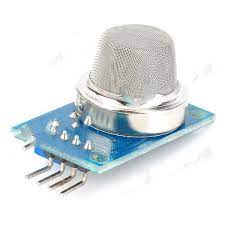
\includegraphics[]{FC22.png}\\
	\caption{\emph{FC22}}
	\label{fig:fc22}
\end{figure}
	\begin{figure}[H]
	\centering
	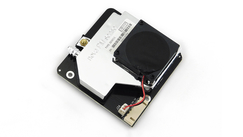
\includegraphics[]{sds011.jpg}\\
	\caption{\emph{SDS011}}
	\label{fig:sds011}
\end{figure}
	\begin{figure}[H]
	\centering
	%\includegraphics[width=1.0\textwidth]{Image.eps}
	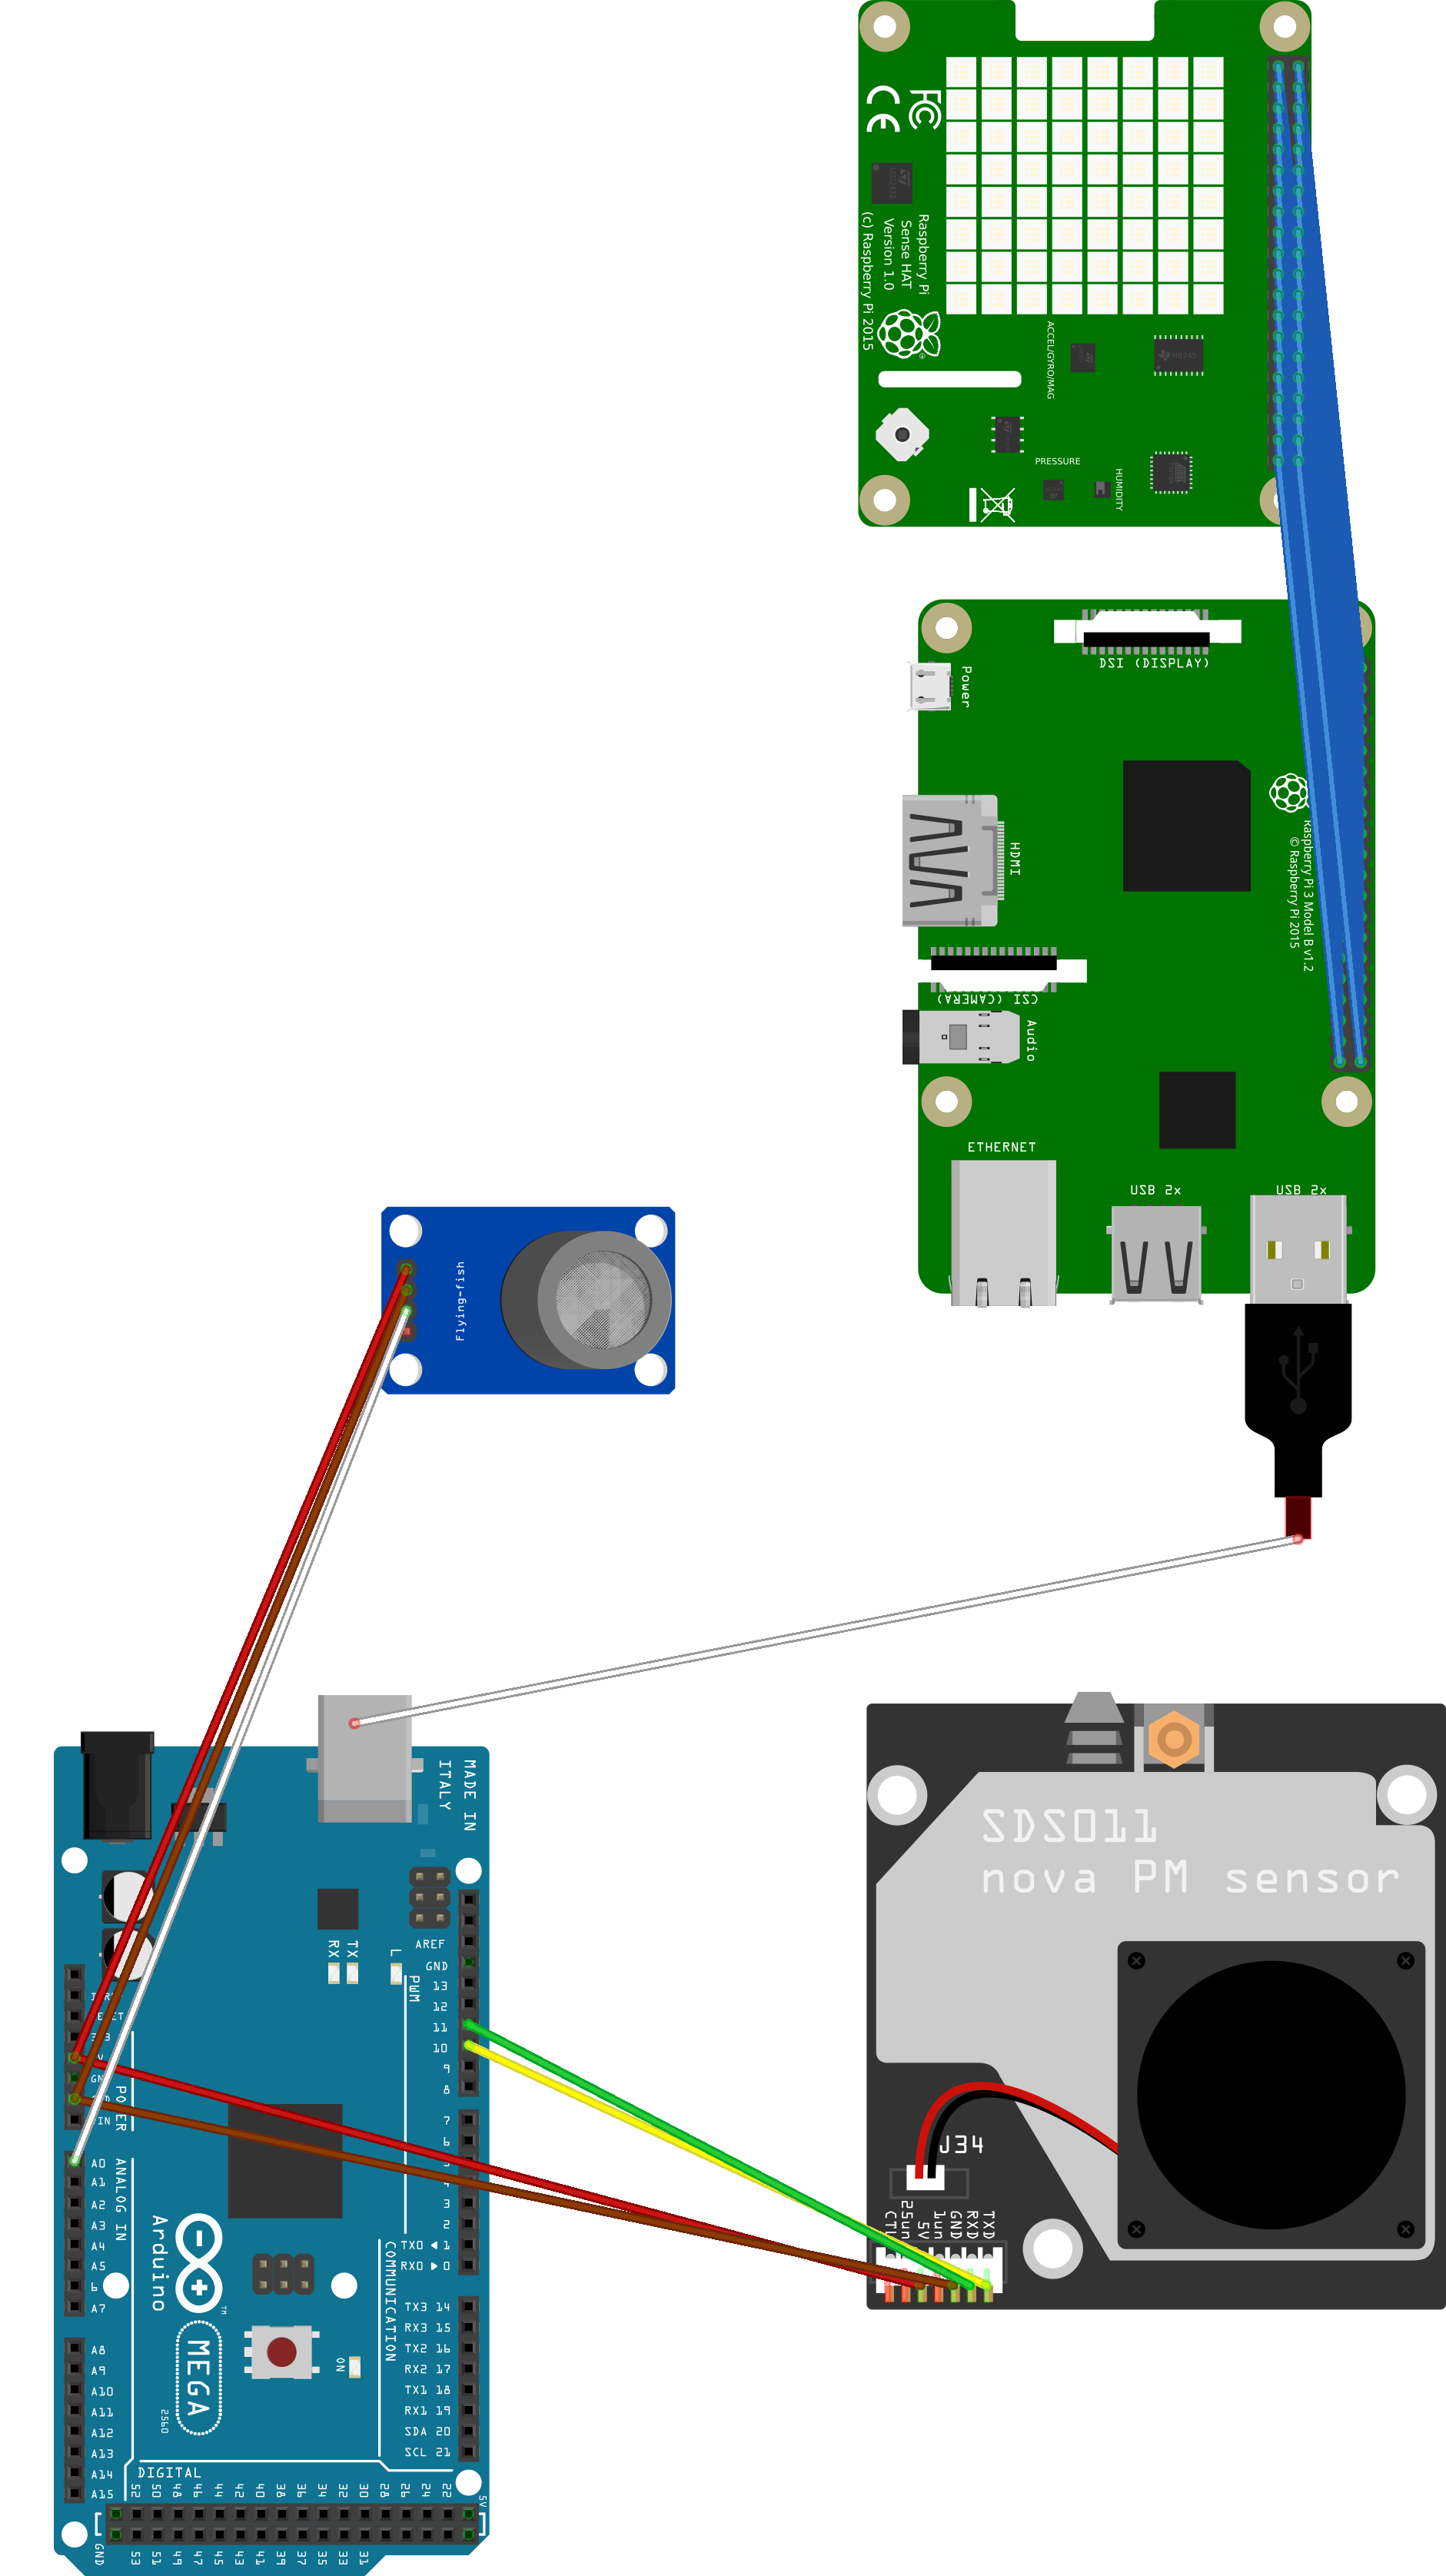
\includegraphics[height=0.95\textheight]{board.png}
	\caption{Depiction of the board}
	\label{fig:board}
\end{figure}
\clearpage
\begin{figure}[!h]
	\centering
	%\includegraphics[width=1.0\textwidth]{Image.eps}
	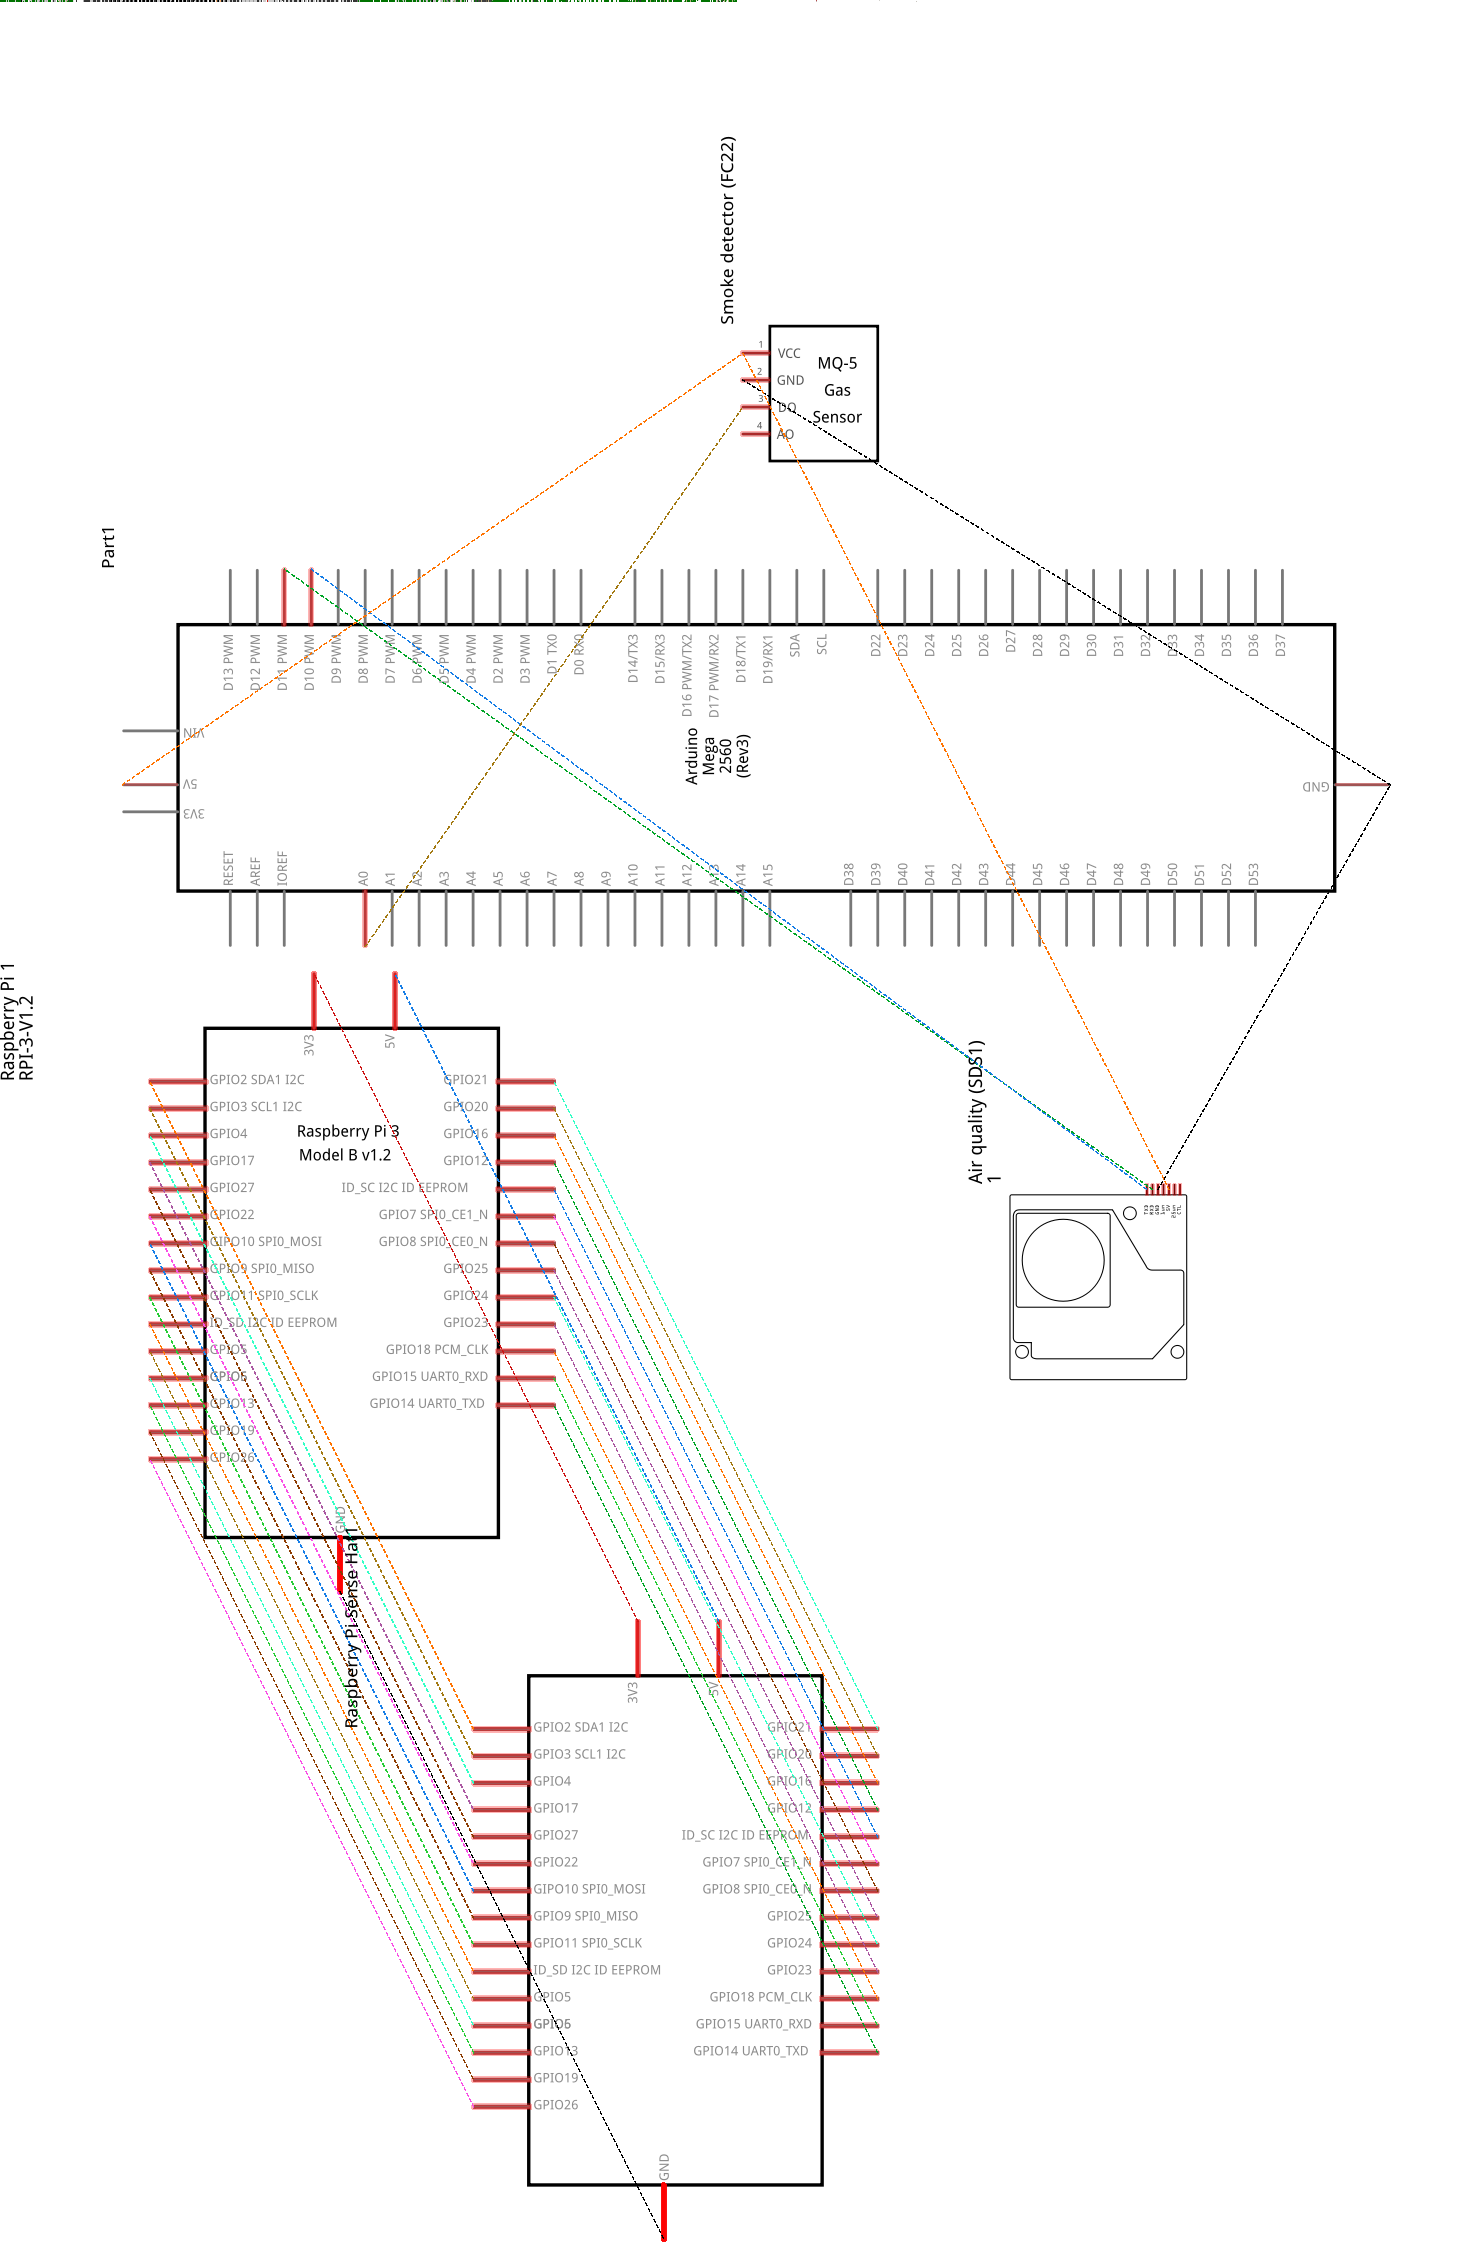
\includegraphics[height=0.95\textheight]{schema.png}
	\caption{Diagram of the board}
	\label{fig:schema}
\end{figure}
\clearpage

\subsection{Presenting Data}
\subsubsection{Display}
A separate unit, carrying a $7''$ display (controlled by a \emph{Raspberry Pi 3B+}), downloads and shows recent and historical data to passers-by and can thus be located in a place where it will be most visible, such as a school hall.\\

Two dashboards are available: an analog display with dials and a minimalist digital ``neon'' display for ease of reading.
\subsubsection{Website}

A web server obtains the data from the \emph{git} archive and displays it in graphs and tables related to different periods of times.

\subsubsection{Repository}

A \emph{git} repository holds the measurements which are saved in \emph{csv} format files.
The file path structure is \texttt{yyyy/mm/dd/type.csv}.

\begin{table}[H]
	\caption{Data format}
	\begin{tabular}{|l|l|l|l|l|}
		
		\hline		
		Data Type   & Format                                                                                                                        & Unit of measurement & \multicolumn{1}{l|}{File type}    & Precision     \\
		\hline		
		\hline		
		Datetime        & \begin{tabular}[c]{@{}l@{}}YYYY-MM-DD hhh:mm:ss\\ \textbf{Caution}: Time is expressed in \\ ``CET'' (+1), italian local \\time\end{tabular} & -                   & -            & -                                          \\ 
		\hline		
		Temperature & decimal                                                                                                                       & $°C$                & \multicolumn{1}{l|}{\texttt{temperature.csv}} & $\pm 0,5°C$  \\
		\hline		
		Humidity    & decimal                                                                                                                       & $\%$                & \multicolumn{1}{l|}{\texttt{humidity.csv}}  & $\pm 4,5\%$   \\ 
		\hline		
		Pressure    & decimal                                                                                                                       & $hPa$                 & \multicolumn{1}{l|}{\texttt{pressure.csv}}   & $\pm 0,1hPa$    \\ 
		\hline		
		Smoke       & decimal                                                                                                                       & $\frac{\mu g}{m^3}$               & \multicolumn{1}{l|}{\texttt{smoke.csv}}     &  $\pm 0,3 \mu\frac{g}{m^3}$    \\ 
		\hline		
		PM10        & decimal                                                                                                                       & $\frac{\mu g}{m^3}$               & \multicolumn{1}{l|}{\texttt{pm10.csv}}     &  $\pm 0,3 \mu\frac{g}{m^3}$      \\ 
		\hline		
		PM2.5       & decimal                                                                                                                       & $\frac{\mu g}{m^3}$               & \multicolumn{1}{l|}{\texttt{pm25.csv}}    &  $\pm 1 \mu\frac{g}{m^3}$      \\
		\hline		
	\end{tabular}
\end{table}
The \emph{repository} also contains a text report about the station operative status (\texttt{report.txt}), and a file which contains the latest data in \texttt{json} format (\texttt{latest.json}).
\clearpage
\begin{figure}[!h]
	\centering
	%\includegraphics[width=1.0\textwidth]{Image.eps}
	
\includegraphics[width=0.95\textwidth]{dash.png}
	\caption{Dashboard}
	\label{fig:dash}
\end{figure}

\begin{figure}[!h]
	\centering
	%\includegraphics[width=1.0\textwidth]{Image.eps}
	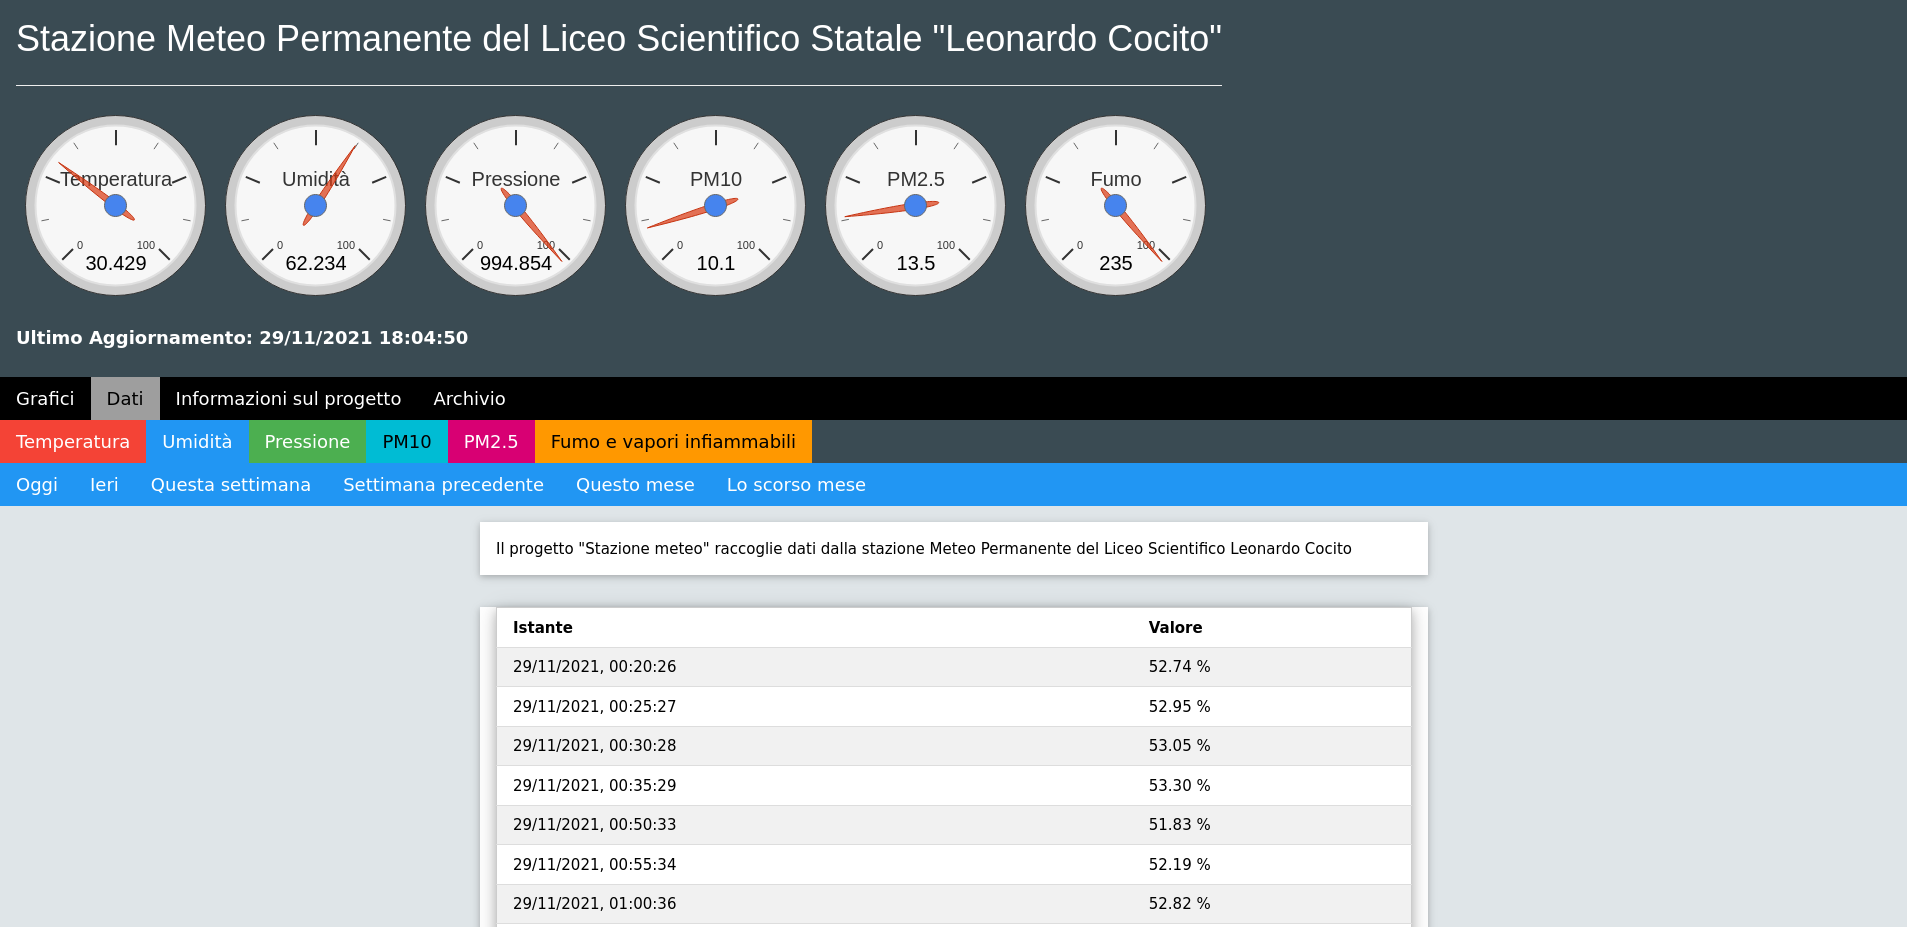
\includegraphics[width=0.95\textwidth]{web.png}
	\caption{Website}
	\label{fig:web}
\end{figure}
\clearpage

\section{Software}
The source code is stored in a git repository at  \url{http://www.github.com/MatMasIt/weatherStation}.\\
The kit contains all the tools necessary for data acquisition, transfer, storage and publication and has been coded with the aid of several programming languages to optimize each task.
	\section{Open data}
The availability of data in an open and standard format makes it possible to carry out comparative surveys, re-elaborations and gives new impetus to the creation of stations that follow the same standard and which can therefore easily join the network and contribute their data to make the collection process even more widespread and effective.
\section{Data relevance}
PM10 has been extensively associated to health concerns \cite{pm101996}, cancer rate increase \cite{pm10} and, more recently, aiding the spread of COVID-19 \cite{pmcovid}.\\
Furthermore, accurate and geographically distributed collection of this kind of data is yet to be achieved, along with the project possibly providing a big meteorological dataset which could be used to enhance existent weather forecasting models and to create new ones, while always being didactically relevant.\\

The data collected in December was compared with the historical dataset of a nearby meteorological station of the Regional Agency for Environmental Protection of Piedmont, and are shown here to highlight their accuracy and usefulness. \\
The Open Source station records the changes in the variables in question with greater decimal precision and frequency, showing they fall within the indicative intervals of the month, taking into account the difference in altitude of the two stations taken into consideration.
\begin{figure}
	\begin{subfigure}{\linewidth}
		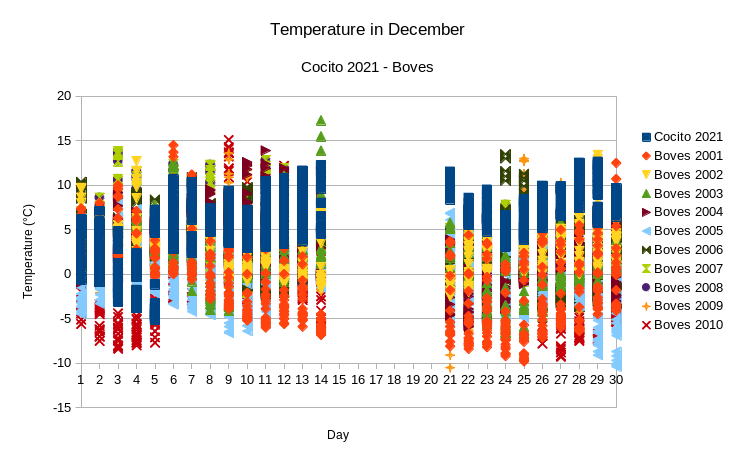
\includegraphics[height=150pt]{graficiBoves/temperature.png}
		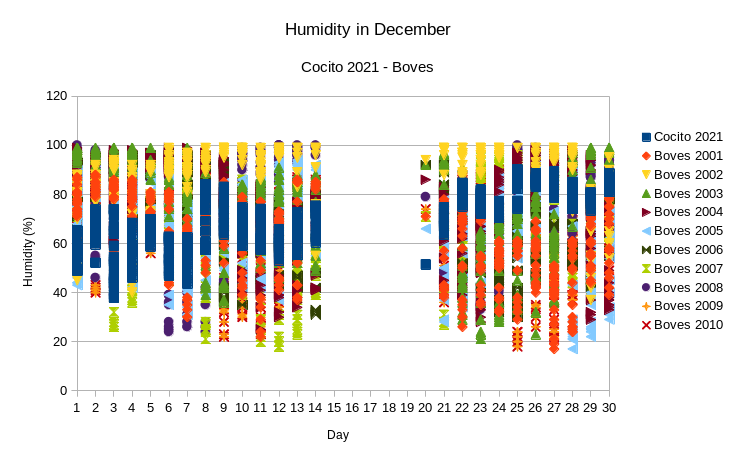
\includegraphics[height=150pt]{graficiBoves/humidity.png}
		\caption{}
	\end{subfigure}\par\medskip
	\begin{subfigure}{\linewidth}
		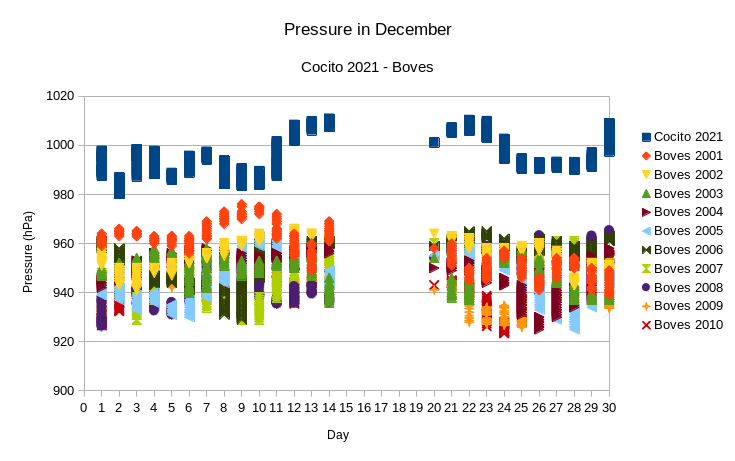
\includegraphics[height=300pt]{graficiBoves/pressure.png}
		\caption{}
	\end{subfigure} 
	\caption{Measurements compared with the historical data of a nearby meteorological station of the Regional Agency for Environmental Protection of Piedmont}
\end{figure}
\vfill
\clearpage
	\begin{table}[H]
	\caption{December 2021 dataset}
	\begin{tabular}{|l|l|@{}c@{}|}
		\hline
		Statistical variable & Calculation & Value\\
		\hline\hline
		Set size & $N$ & \begin{tabular}{c|p{2cm}} Temperature & $5005$ \\ \hline Humidity & $5005$ \\ \hline Pressure & $5002$ \\ \hline PM10 & $4998$\\ \hline PM2,5& $4998$\\ \hline Smoke and flammable vapors& $4998$ \end{tabular} \\
		\hline
		Maximum & $max$ & \begin{tabular}{c|p{2cm}} Temperature & $21,13°C$ \\ \hline Humidity & $90,85 \%$ \\ \hline Pressure & $ 	1'011,03 hPa$ \\ \hline PM10 & $143,70\frac{\mu g}{m^3}$\\ \hline PM2,5& $156,10\frac{\mu g}{m^3}$\\ \hline Smoke and flammable vapors& $420,00\frac{\mu g}{m^3}$ \end{tabular} \\
		\hline
		Mimimum & $min$ & \begin{tabular}{c|p{2cm}} Temperature & $-7,34°C$ \\ \hline Humidity & $34,97 \%$ \\ \hline Pressure & $980,04 hPa$ \\ \hline PM10 & $4\frac{\mu g}{m^3}$\\ \hline PM2,5& $5,40\frac{\mu g}{m^3}$\\ \hline Smoke and flammable vapors& $130,00\frac{\mu g}{m^3}$ \end{tabular} \\
		\hline
		Arithmetic average & $\mu=\frac{\sum_{i=1}^{N}x_i}{N}$ & \begin{tabular}{c|p{2cm}} Temperature & $4,96°C$ \\ \hline Humidity & $68,5 \%$ \\ \hline Pressure & $995,3 hPa$ \\ \hline PM10 & $32,99 \frac{\mu g}{m^3}$\\ \hline PM2,5& $41,92 \frac{\mu g}{m^3}$\\ \hline Smoke and flammable vapors& $178,14 \frac{\mu g}{m^3}$ \end{tabular} \\
		\hline
		Standard deviation & 	$\sigma _{X}={\sqrt {\frac {\sum \limits _{i=1}^{N}(x_{i}-{\bar {x}})^{2}}{N-1}}}
		$ & \begin{tabular}{c|p{2cm}} Temperature & $3,53°C$ \\ \hline Humidity & $10,48 \%$ \\ \hline Pressure & $8,25 hPa$ \\ \hline PM10 & $24,59 \frac{\mu g}{m^3}$\\ \hline PM2,5& $27,01 \frac{\mu g}{m^3}$\\ \hline Smoke and flammable vapors& $17,81 \frac{\mu g}{m^3}$ \end{tabular}  \\
		\hline
		Variation coefficient & 	$ \sigma ^{*}={\frac {\sigma }{|\mu |}}$ & \begin{tabular}{c|p{2cm}} Temperature & $0,71$ \\ \hline Humidity & $0,15$ \\ \hline Pressure & $8,28\cdot10^{-3}$ \\ \hline PM10 & $0,74$\\ \hline PM2,5& $0,64$\\ \hline Smoke and flammable vapors& $0,1$ \end{tabular} \\
		\hline
		Mode (integer)& 	$Mo$ & \begin{tabular}{c|p{2cm}} Temperature & $6 °C$ \\ \hline Humidity & $74 \%$ \\ \hline Pressure & $995 hPa$ \\ \hline PM10 & $22\frac{\mu g}{m^3}$\\ \hline PM2,5&  $45\frac{\mu g}{m^3}$\\ \hline Smoke and flammable vapors&  $181\frac{\mu g}{m^3}$\end{tabular} \\
		\hline
	\end{tabular}
\end{table}
\section{Conclusions}
In conclusion, the team has laid the groundwork and the instructions for the easy construction of weather and air quality monitoring stations, in a didactically integrated fashion which could be pursued by many schools and produce great value both in didactic terms and result-wise, given the many applications that these stations can have.
\clearpage
\printbibliography
\end{document}